\documentclass[11pt,a4paper]{scrartcl}
\usepackage[utf8]{inputenc}
\usepackage[T1]{fontenc}
\usepackage[ngerman]{babel}
\usepackage{geometry}
\usepackage{graphicx}
\usepackage{hyperref}
\usepackage{caption}
\usepackage{float}
\usepackage{minted}
\usepackage{parskip}
%\geometry{top=25mm,bottom=25mm,left=25mm,right=25mm}

\title{Aufgabe 3: Addressierungsbeispiel}
\author{Florian Breitwieser \\ \& Jakob Zimmermann}
\date{\today}

\begin{document}
\maketitle

\section{Einleitung}
Dieses Dokument beschreibt die Umsetzung des Adressierungsbeispiels als Teil der Aufgabe 3. Es fasst die Architektur des Address-Slave und des Address-Master zusammen, dokumentiert die Simulation und beschreibt Metastabilitätseffekte.

\newpage
\section{Aufgabenstellung}
Ziel ist die Implementierung eines adressierbaren LED-Slave-Moduls für das iceduino-Board und eines synthetisierbaren Masters, der die LEDs in einem Lauflicht ansteuert. Die Abgabenanforderungen umfassen:
\begin{itemize}
  \item Slave Code und erläuternder Text zur Funktion
  \item Slave Testbench Code und erläuternder Text zur Funktion, inklusive asserts und Hinweis auf nicht-synthetisierbaren Testbench-Code
  \item Simulation Slave mit Testbench (Screenshot + Analyse)
  \item Master Blockschaltbild inkl. Slave-Anbindung
  \item Master Code
  \item Master Simulation mit Slave
  \item Erläuterung der Simulationsergebnisse und Master-Statemachine
  \item Metastabilitätsbetrachtung: Ursache, Auswirkung und Vermeidung
\end{itemize}

\newpage
\section{Addr\_Slave Code}
Der folgende Code zeigt das Low-Level-Verhalten des Slave-Moduls. Es verarbeitet den Reset, liest die Adresse und schreibt bei gesetztem \texttt{we} das Datensignal \texttt{d} in das entsprechende LED-Register.

\begin{minted}[linenos,breaklines,fontsize=\small]{vhdl}
library ieee;
use IEEE.std_logic_1164.all;
use IEEE.numeric_std.all;

entity addr_slave is
    port(
        clk: in std_logic;
        we : in std_logic;
        d : in std_logic;
        rst : in std_logic;
        addr : in std_logic_vector(2 downto 0);
        leds : out std_logic_vector(7 downto 0)
    );
end entity;

architecture addr_slave_a of addr_slave is
begin
    process(clk, rst) is
    begin
        if rst = '1' then
            leds <= (others => '0');
        elsif rising_edge(clk) then
            if we = '1' then
                leds(to_integer(unsigned(addr))) <= d;
            end if;    
        end if;
    end process;
end architecture addr_slave_a;
\end{minted}

Bei steigender Flanke des Taktsignals \texttt{clk} und aktivem Reset (\texttt{rst = '1'}) werden alle LEDs gelöscht. Wenn \texttt{we} gesetzt ist, wird das Datenbit \texttt{d} an der Position geschrieben, die durch die Adresse \texttt{addr} bestimmt wird. Die LEDs werden als 8-Bit-Vektor ausgegeben, wobei jedes Bit eine LED repräsentiert.

\newpage
\section{Addr\_Slave Testbench}
Die Testbench prüft die korrekte Adressierung des Slave-Moduls für mehrere Adressen und enthält Assert-Anweisungen für die LED-Ausgabe.

\begin{minted}[linenos,breaklines,fontsize=\small]{vhdl}
library ieee;
use IEEE.std_logic_1164.all;
use IEEE.numeric_std.all;

entity addr_slave_tb is
end entity;

architecture addr_slave_tb_a of addr_slave_tb is
    signal clk : std_logic := '0';
    signal we : std_logic := '0';
    signal d : std_logic := '0';
    signal reset : std_logic := '0';
    signal addr : std_logic_vector(2 downto 0) := (others => '0');
    signal leds : std_logic_vector(7 downto 0) := (others => '0');
begin
    clk <= not clk after 10 ns; -- 50 MHz

    addr_slave_instance : entity work.addr_slave
        port map(
            clk => clk,
            we => we,
            d => d,
            reset => reset,
            addr => addr,
            leds => leds
        );

    process is
    begin
        reset <= '1';
        wait for 30 ns;
        reset <= '0';

        addr <= (others => '0');
        wait for 10 ns;
        d <= '1';
        we <= '1';

        wait for 80 ns;
        assert (leds = "00000001") report "R1: LEDS falsch" severity error;
        assert (addr = "000") report "R1: b0 falsch" severity error;
        report "R1: OK" severity note;
        we <= '0';
        wait for 1 ns;
        d <= '0';

        wait for 200 ns;
        addr <= (others => '1');
        wait for 10 ns;
        d <= '1';
        we <= '1';

        wait for 80 ns;
        assert (leds = "10000001") report "R2: LEDS falsch" severity error;
        assert (addr = "111") report "R2: addr falsch" severity error;
        report "R2: OK" severity note;
        we <= '0';
        wait for 1 ns;
        d <= '0';

        wait for 200 ns;
        addr <= "010";
        wait for 10 ns;
        d <= '1';
        we <= '1';

        wait for 80 ns;
        assert (leds = "10000101") report "R3: LEDS falsch" severity error;
        report "R3: OK" severity note;
        we <= '0';
        wait for 200 ns;
        d <= '0';
    end process;
end architecture addr_slave_tb_a;
\end{minted}

Alle Asserts konnten erfolgreich durchlaufen werden. Der addr-slave funktioniert einwandfrei. 

Alle 'wait' und 'after' Anweisungen sind nicht-synthetisierbar und dienen ausschließlich der Simulation.

\begin{figure}[!htbp]
  \centering
  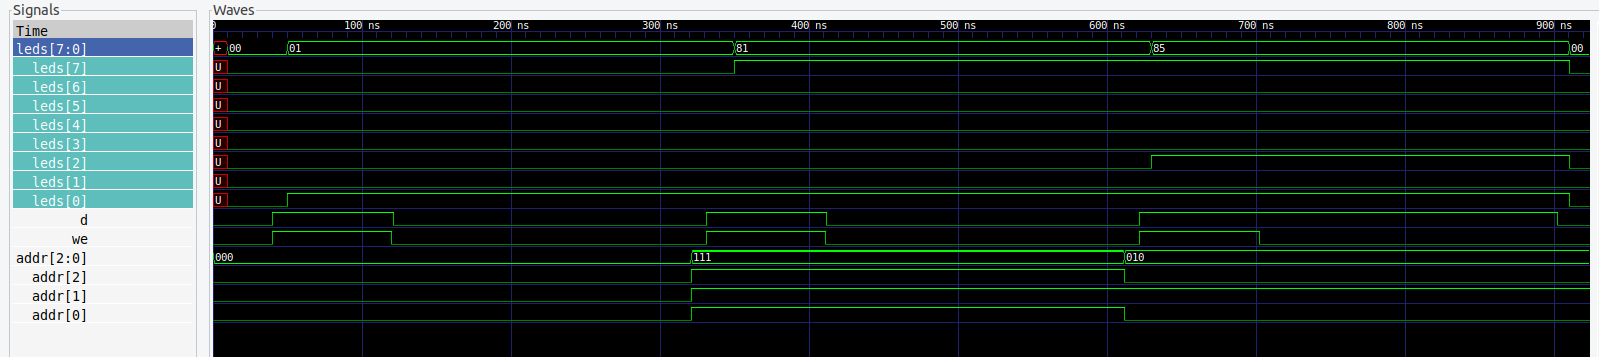
\includegraphics[width=\textwidth]{resources/sim_addrslave.png}
  \caption{Simulation des Address-Slave mit Testbench}
\label{fig:slave-sim}  
\end{figure}

Die Simulation zeigt die korrekte Adressierung und LED-Ausgabe für die getesteten Adressen. Bei Adresse '000' leuchtet die erste LED, bei '111' die letzte LED, und bei '010' die dritte LED. Alle Asserts bestätigen die erwarteten Ergebnisse.

\newpage
\section{Master Architektur und Code}

\begin{figure}[h]
  \centering
  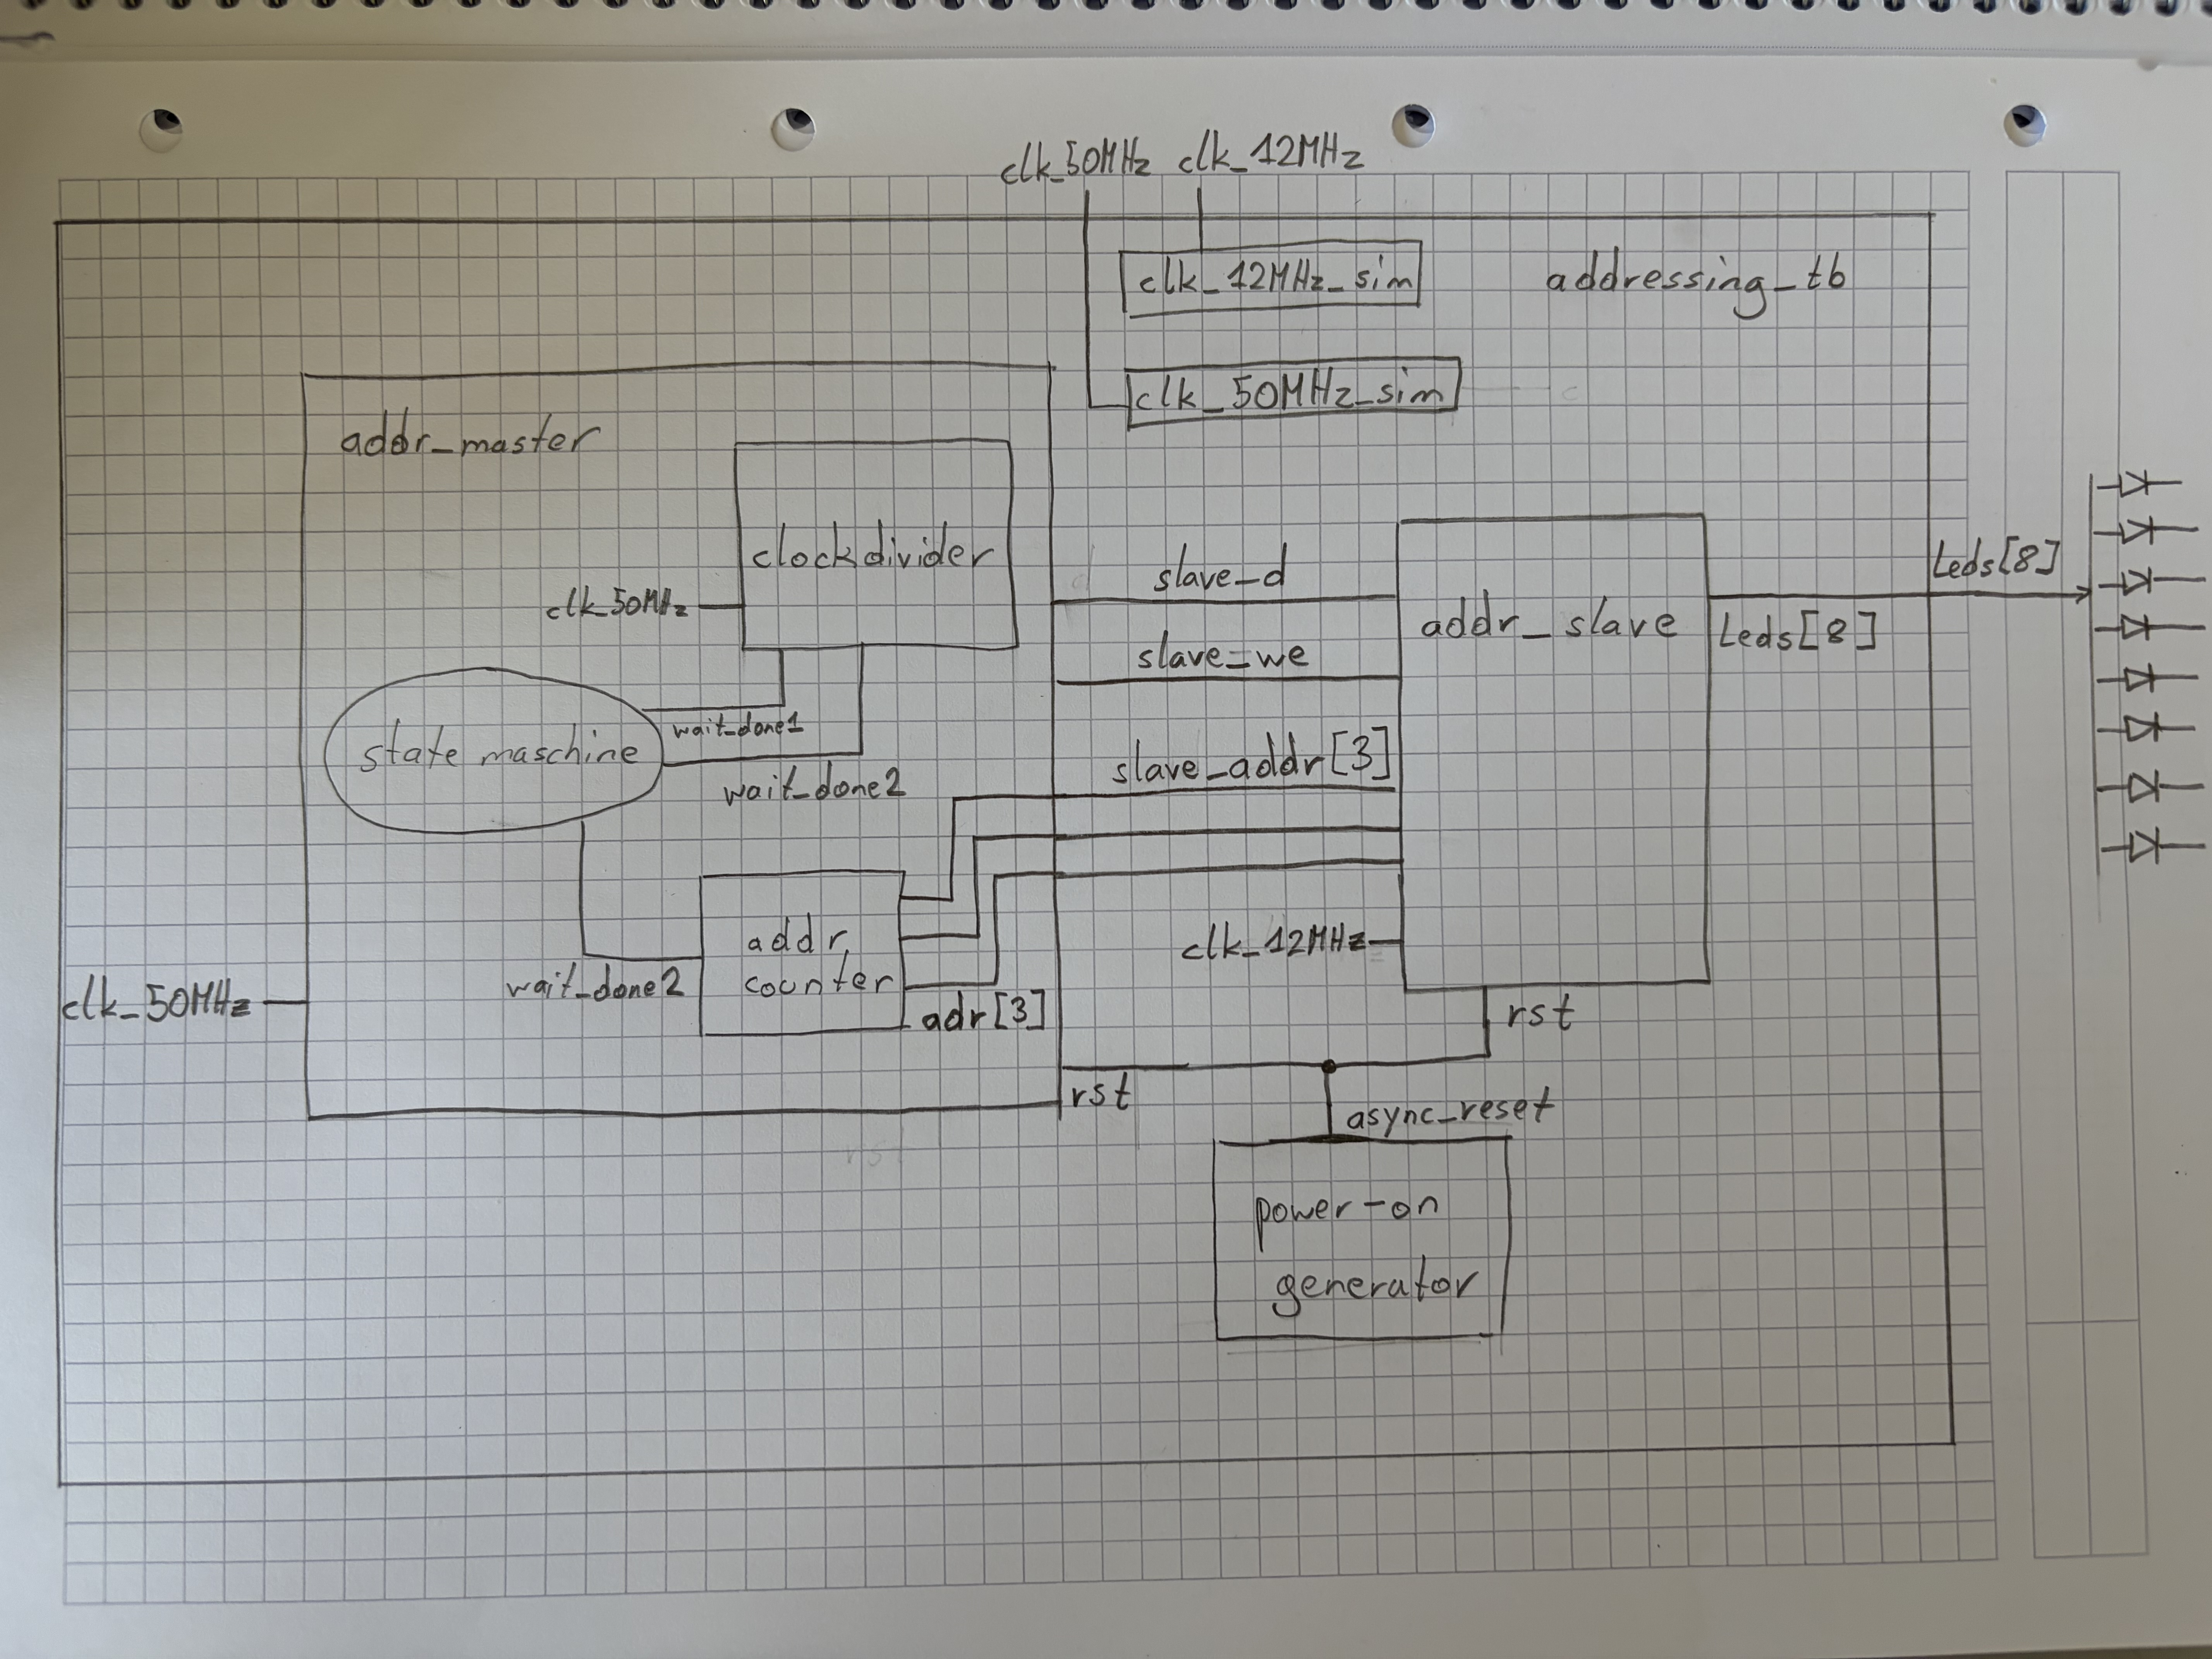
\includegraphics[width=\textwidth]{resources/system_overview.jpeg}
  \caption{Blockschaltbild des Address-Master und Slave-Anbindung}
\label{fig:master-block}  
\end{figure}

Das Bild zeigt die Zusammenschaltung des Address-Master mit dem Address-Slave. Der Master generiert die Signale \texttt{adr}, \texttt{we} und \texttt{d}, die direkt an den Slave weitergegeben werden. Ein Power-On-Reset-Generator sorgt für einen definierten Reset-Zustand nach FPGA-Neustart.

Der \texttt{addr\_master} erzeugt die Steuerungsimpulse für den Slave. Er durchläuft die Adressen \texttt{000} bis \texttt{111} und schaltet jeweils eine LED ein, wartet dann eine definierte Verzögerungszeit, schaltet ab und geht zur nächsten Adresse.



\begin{minted}[linenos,breaklines,fontsize=\small]{vhdl}
entity addr_master is
    generic (
        variable_delay : integer := 12500000
    );
    port(
        clk : in std_logic;
        rst : in std_logic;
        adr : out std_logic_vector(2 downto 0);
        we : out std_logic;
        d : out std_logic
    );
end entity;

architecture addr_master_a of addr_master is
    type state_type is (START, LON, LOFF);
    signal state : state_type := START;
    signal cnt : integer range 0 to 12500000 := 0;
    signal adr_reg : unsigned(2 downto 0) := "000";
    signal delay_cnt : integer range 0 to variable_delay := 0;
    signal slave_we : std_logic := '0';
    signal slave_d : std_logic := '0';
    signal delay_cnt2 : integer range 0 to 20000 := 0;
    signal wait_done1 : std_logic := '0';
    signal wait_done2 : std_logic := '0';
begin
        
    process (clk, rst)
        begin

        if rst = '1' then
            state <= START;
            slave_we <= '0';
            slave_d <= '0';
            wait_done1 <= '0';
            wait_done2 <= '0';
        elsif rising_edge(clk) then
                case state is
                    when START =>
                        state <= LON;
                        wait_done1 <= '0';
                        wait_done2 <= '0';
                    when LON =>
                        slave_d <= '1';
                        if delay_cnt = 0 then
                            slave_we <= '1';
                            delay_cnt <= delay_cnt + 1;
                        elsif delay_cnt = 10 then
                            slave_we <= '0';
                            delay_cnt <= delay_cnt + 1;
                        elsif delay_cnt = variable_delay then
                            delay_cnt <= 0;
                            wait_done1 <= '1';
                        else
                            delay_cnt <= delay_cnt + 1;
                        end if;
                        
                        if wait_done1 = '1' then
                            state <= LOFF;
                            wait_done1 <= '0';
                        end if;
                    when LOFF =>
                        slave_d <= '0';
                        slave_we <= '1';
                        
                        if delay_cnt2 = 10 then
                            delay_cnt2 <= 0;
                            slave_we <= '0';
                            wait_done2 <= '1';
                        else
                            delay_cnt2 <= delay_cnt2 + 1;
                        end if; 
                        
                        if wait_done2 = '1' then
                            if adr_reg = "111" then
                                adr_reg <= "000";
                            else
                                adr_reg <= adr_reg + 1;
                            end if;

                            state <= LON;
                            wait_done2 <= '0';
                        end if;
                end case;
        end if;
    end process;

    adr <= std_logic_vector(adr_reg);
    d <= slave_d;
    we <= slave_we;
end architecture addr_master_a;
\end{minted}

Der Master verwendet einen Zustandsautomaten mit den Zuständen:
\begin{itemize}
  \item \textbf{START}
  \item \textbf{LON} (LED einschalten)
  \item \textbf{LOFF} (LED ausschalten)
\end{itemize}

Das folgende Zustandsdiagramm zeigt die Übergänge zwischen den Zuständen.

\begin{figure}[!htbp]
  \centering
  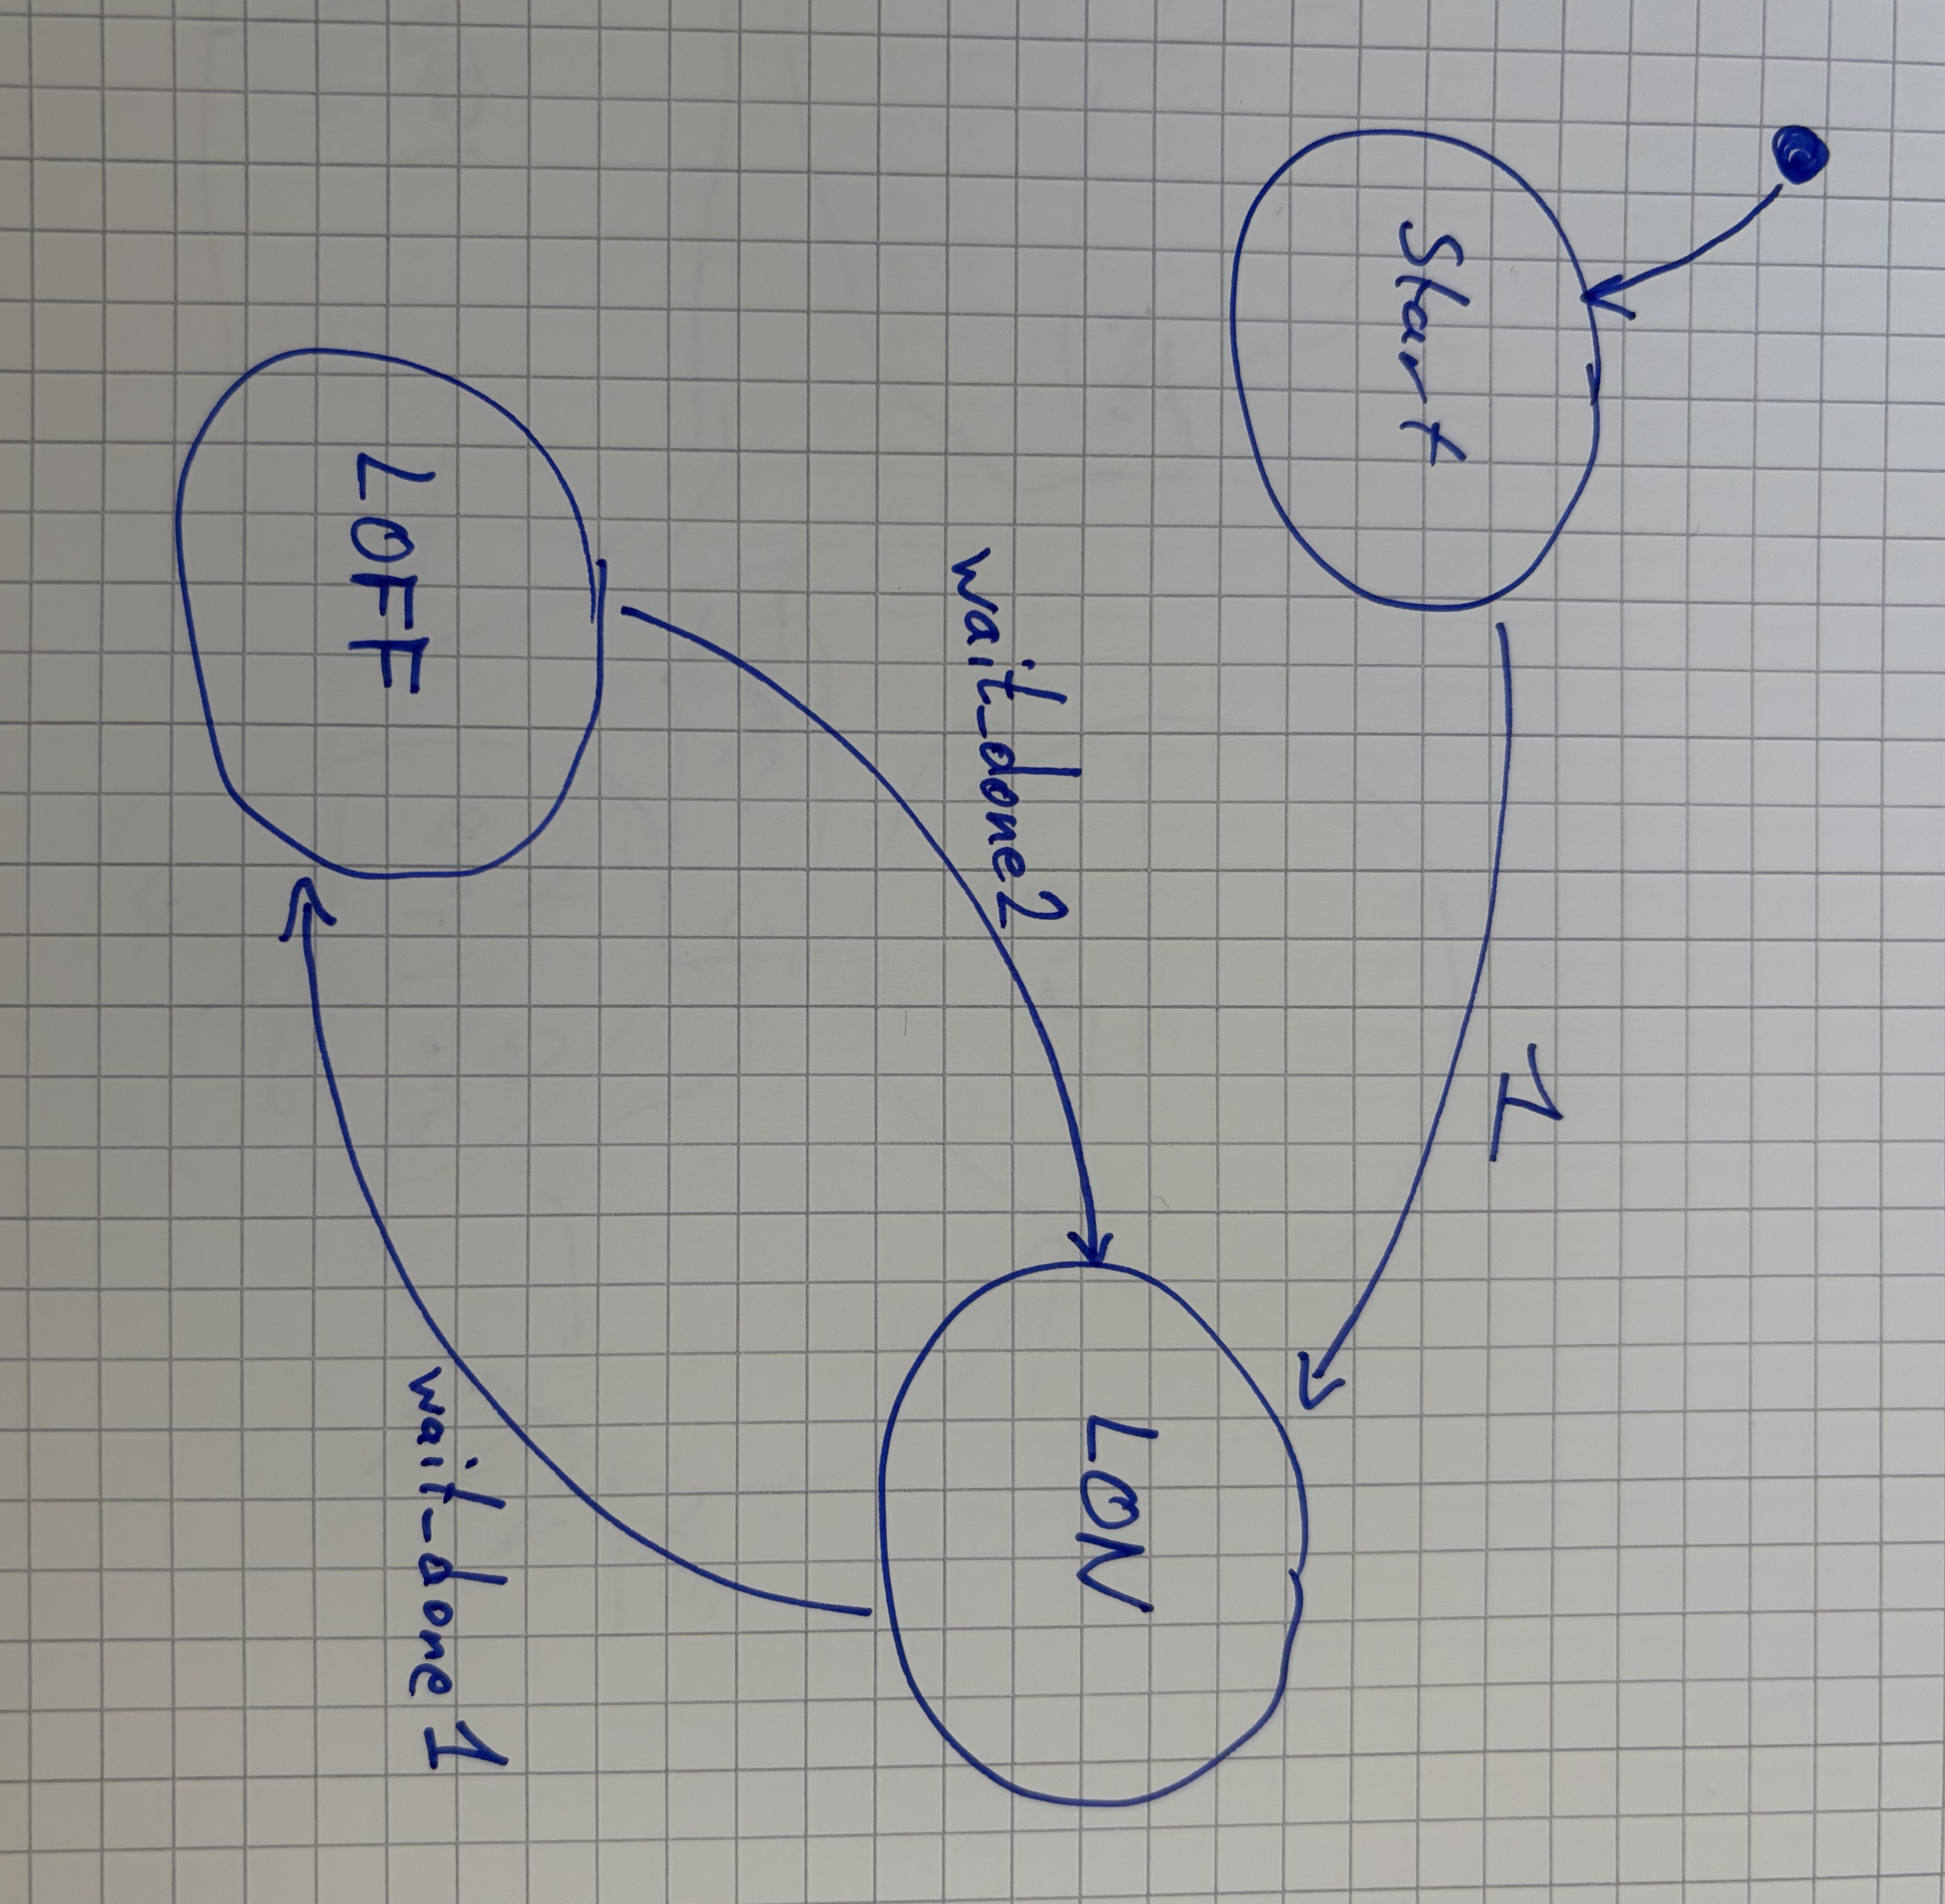
\includegraphics[scale=0.1, angle=90]{resources/state_maschine.jpeg}
  \caption{Zustandsdiagramm des Address-Master}
\label{fig:master-fsm}
\end{figure}

\newpage
\section{Testbench}
Die Testbench \texttt{addressing\_tb.vhd} implementiert die Addressing-Simulation mit verkürztem Delay.

\begin{minted}[linenos,breaklines,fontsize=\small]{vhdl}
entity addressing_tb is
    generic (
        variable_delay : integer := 500
    );

    port(
    clk_12MHz : in std_logic;
    clk_50MHz : in std_logic;
    leds : out std_logic_vector(7 downto 0)
    );
end entity;

architecture addressing_tb_a of addressing_tb is
    signal async_reset : std_logic := '1';
    signal slave_we : std_logic := '0';
    signal slave_d : std_logic := '0';
    signal slave_addr : std_logic_vector(2 downto 0) := "000";
    signal clk_12MHz_sim : std_logic := '0';
    signal clk_50MHz_sim : std_logic := '0';
    signal counter : unsigned(7 downto 0) := (others => '0');
    begin
        
        clk_12MHz_sim <= not clk_12MHz_sim after 41.666666 ns;
        clk_50MHz_sim <= not clk_50MHz_sim after 10 ns;
    
        process(clk_12MHz_sim) is
            variable cnt : unsigned(7 downto 0) := (others => '0');
        begin
            if rising_edge(clk_12MHz_sim) then
                if cnt < 255 then
                    cnt := cnt + 1;
                    counter <= cnt;
                    async_reset <= '1';
                else 
                    counter <= cnt;
                    async_reset <= '0';
                end if;
            end if;
        end process;

    addr_master_instance : entity work.addr_master
    generic map(
        variable_delay => variable_delay
    )
    port map(
        clk => clk_50MHz_sim,
        rst => async_reset,
        adr => slave_addr,
        we => slave_we,
        d => slave_d
    );

    addr_slave_instance : entity work.addr_slave
    port map(
        clk => clk_12MHz_sim,
        we => slave_we,
        d => slave_d,
        rst => async_reset, 
        addr => slave_addr,
        leds => leds
    );


    end architecture addressing_tb_a;
\end{minted}

\begin{figure}[!htbp]
  \centering
  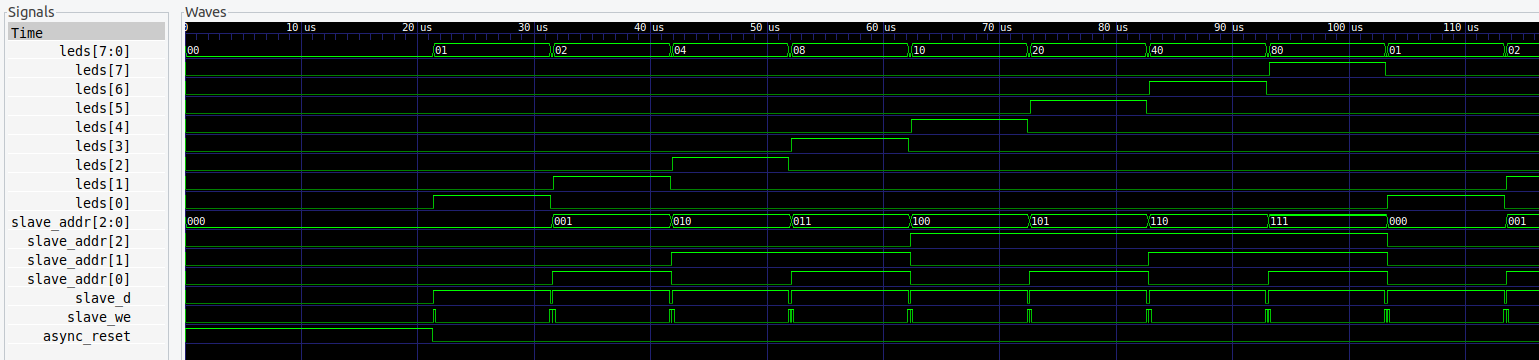
\includegraphics[width=\textwidth, angle=0]{resources/sim1.png}
  \caption{Simulation des Address-Master mit Slave}
\label{fig:master-fsm}
\end{figure}
Die Simulation zeigt die korrekte Funktionalität des Masters und Slaves. Der Master durchläuft die Adressen von '000' bis '111', schaltet die entsprechenden LEDs ein und aus.

\newpage
\section{Metastabilität}
Flip-Flops können metastabil werden, wenn asynchrone Eingangssignale sehr nahe an der aktiven Flanke des Taktes wechseln. In diesem Zustand bleibt das Flip-Flop für eine unbestimmte Zeit in einem undefinierten Spannungsbereich, was zu Glitches, Fehlern oder falschen Datenweiterleitungen führen kann.

\subsection{Ursachen}
\begin{itemize}
  \item asynchrone Signaländerungen nahe am Taktflankenzeitpunkt
  \item nicht eingehaltene Setup- und Hold-Zeiten
  \item fehlende Synchronisation zwischen verschiedenen Taktdomänen
\end{itemize}

\subsection{Auswirkungen}
\begin{itemize}
  \item fehlerhafte Signalausgabe
  \item unvorhersehbares Verhalten von State Machines
  \item sporadische Systemausfälle
\end{itemize}

\subsection{Vermeidung}
\begin{itemize}
  \item Synchronisationsstufen (z. B. zwei Flip-Flops hintereinander)
  \item ausreichende Setup- und Hold-Zeiten
  \item Verwendung von Taktdomänen-Grenzen und Cross-Clock-Handshake
\end{itemize}

\end{document}